\documentclass{myproject}

\graphicspath{{../Figures/}}

% title setup
\title{\vspace*{-1cm}Solving the Inviscid Burgers' Equation Numerically}
\date{}
\author{
    Andre Gormann\\
    agormann@sfu.ca
    \and
    Ethan MacDonald\\
    jem21@sfu.ca
}

% bibliography
\addbibresource{references.bib}

\renewcommand*{\thefootnote}{[\arabic{footnote}]}

\begin{document}

% title creation
\maketitle
\vspace*{-1cm}
% contents
\tableofcontents

% document 
\section{Introduction}

The 1-D inviscid Burgers' equation is a first-order hyperbolic partial differential equation (PDE) of the form
\begin{equation}\label{burgers_long}
    \partial_t u(x,t) + u(x,t)\partial_xu(x,t) = 0
\end{equation}
where $u \in C^1(\Omega)$, and $x,t \in \Omega \subset \R\times\R^+$. Note that a more compact form of \eqref{burgers_long} is $u_t + uu_x = 0$. The latter formulation is what is commonly seen in literature. 

This equation has a brother named the \emph{viscous} Burgers' equation (or simply referred to as Burgers' equation), which takes the form
\begin{equation}\label{burgers_viscous}
    u_t + uu_x = \epsilon u_{xx}
\end{equation}
where $\epsilon > 0$ is the diffusion coefficient. We mention this because the inviscid Burgers' equation can be interpreted as resulting from letting $\epsilon \to 0$ in \eqref{burgers_viscous}. This is important because it informs us what the `correct' behavior of \eqref{burgers_long} should be.

The quasilinear equation \eqref{burgers_long} is not the only formulation of the inviscid Burgers' equation, and in a certain sense it is actually the `wrong' one to study. This is because under a few reasonable assumptions, a completely smooth initial profile modeled by \eqref{burgers_long} will devolve into a discontinuous one in finite time. This is unsettling because then \eqref{burgers_long} fails to hold; the partial derivative of a discontinuous function does not exist!

Instead, we rewrite \eqref{burgers_long} as
\begin{equation}\label{burgers_conservative}
    u_t + f(u)_x = 0
\end{equation}
where
\begin{equation}
    f(u) = \frac{1}{2}u^2
\end{equation}
is known as the flux function. This is known as the conservation form of the inviscid Burgers' equation. If we integrate \eqref{burgers_conservative} over $[a,b]$, where $[a,b] \subset \Omega$, then we get
\begin{equation}\label{burgers_integral}
    \frac{d}{dt}\int_{a}^{b} u(x,t) dx = f(u(a,t)) - f(u(b,t))
\end{equation}
where we have exchanged differentiation and integration. The form \eqref{burgers_integral} is known as the integral form of \eqref{burgers_conservative}, and it is where the `conservative' notion comes from.

Importantly, this integral form has no problems admitting profiles $u$ with spatial discontinuities (we assume it is not also discontinuous in time). It is this formulation (not \eqref{burgers_long}) that we will be studying and developing our numerical schemes for. 

\section{Theory}

yahoo theory

\subsection{Finite Volume Methods for Conservation Laws}

i heart fvm

\subsection{The REA Algorithm}

more like diarrhea amirite

\subsection{The Riemann Problem}

i got 99 problems and riemann is one

\begin{figure}
    \centering
    \begin{subfigure}{.48\textwidth}
        \centering
        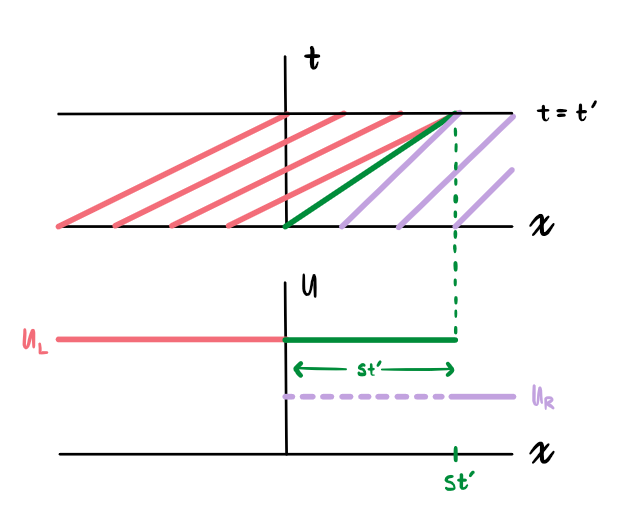
\includegraphics[width=1.0\textwidth]{riemann_shockwave.png}
        \caption{caption 1}
        \label{fig:shock}
    \end{subfigure}\hfill
    \begin{subfigure}{.48\textwidth}
        \centering
        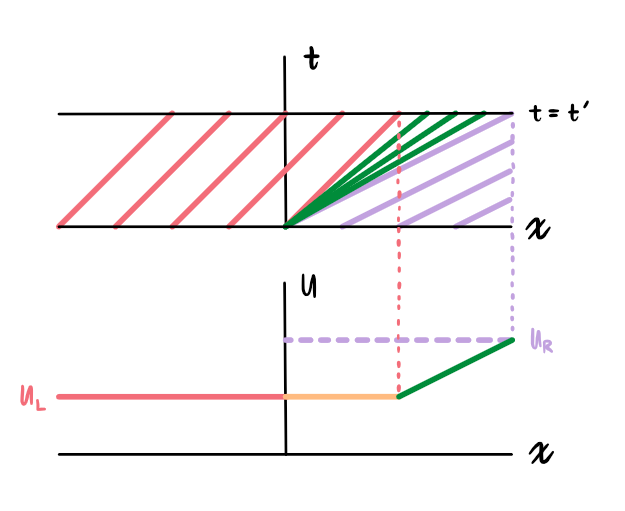
\includegraphics[width=1\textwidth]{riemann_rarefaction.png}
        \caption{caption 2}
        \label{fig:rarefaction}
    \end{subfigure}
    \caption{main caption}
    \label{fig:riemann_discontinuities}
\end{figure}

\subsection{Convergence}



\subsection{High-Resolution Methods}

shit i dont fully understand how to implement

\section{Experiments}

where our code crashed and burns

\subsection{`Easy' Problems}

\begin{itemize}
	\item \textbf{Riemann Problem}
	
	The Riemann Problem studies the formation of shocks. The initial condition is as follows
	\begin{equation}
		u(x,0) = 
	    \begin{cases}
	      	u_L & \text{if } x < 0 \\
			u_R & \text{if } x \geq 0
	    \end{cases}
	\end{equation}
	where $u_L > u_R$. In our experiment, we set $u_L = 1$ and $u_R = 0$. The true solution is
	\begin{equation}
		u(x,t) = 
	    \begin{cases}
	      	u_L = 1 & \text{if } x < st \\
			u_R = 0 & \text{if } x \geq st
	    \end{cases}
	\end{equation}
	where \[s = \frac{u_L + u_R}{2}\ = \frac{1}{2}\] is the speed of the shock. This is known as the Rankine-Hugoniot condition. In our experiment, we shifted right spacially by $\pi$ and used the boundaries $[0, 2\pi]$. This made our plots more consistent with the harder problems, which are all $[0, 2\pi]$ periodic.
	
	RESULTSSSSSSSSSSSSSSSS
	
	\item \textbf{Rarefaction Wave}
	
	If we take the Riemann Problem but instead have $u_L < u_R$, a shock will not form. In this case we get what is called a rarefaction wave. In our experiment, we set $u_L = 0$ and $u_R = 1$. The true solution is
	\begin{equation}
		u(x,t) = 
	    \begin{cases}
	      	u_L = 0 & \text{if } x \leq {u_L}t \\
			\frac{x}{t} & \text{if } {u_L}t < x < {u_R}t \\
			u_R = 1 & \text{if } x \geq {u_R}t
	    \end{cases}
	\end{equation}
	
\end{itemize}

\subsection{`Hard' Problems}

\begin{itemize}
	\item \textbf{Sinusoidal Initial Conditions}
	
	We experimented with the following IVP
	\begin{equation}
	    \begin{cases}
	      	u_t + uu_x = 0, \: x \in [0, 2\pi], \: t>0 \\
			u(x,0) = sin(x) \\
			u(0,t) = u(2\pi,t) \: \forall t
	    \end{cases}
	\end{equation}
	
	\item \textbf{Squared Sinusoidal Initial Conditions}
	
	We experimented with the following IVP
	\begin{equation}
	    \begin{cases}
	      	u_t + uu_x = 0, \: x \in [0, 2\pi], \: t>0 \\
			u(x,0) = sin^2(\frac{x}{2}) \\
			u(0,t) = u(2\pi,t) \: \forall t
	    \end{cases}
	\end{equation}
	
	\item \textbf{Squared Sinusoidal Initial Conditions}
	
	We experimented with the following IVP
	\begin{equation}
	    \begin{cases}
	      	u_t + uu_x = 0, \: x \in [0, 2\pi], \: t>0 \\
			u(x,0) = g(x) \\
			u(0,t) = u(2\pi,t) \: \forall t
	    \end{cases}
	\end{equation}
	where
	\begin{equation}
		g(x) = 
	    \begin{cases}
	      	1 & \text{if } x \in [\frac{\pi}{2}, \frac{3\pi}{2}] \\
			0 & \text{otherwise} 
	    \end{cases}
	\end{equation}
		
\end{itemize}

\section{Conclusion}

this shit was way harder than i thought it would be

\newpage
\appendix
\section{Appendix}
\subsection{Code}

All project code can be found on our GitHub page: \url{https://github.com/agormann/MACM416-project}. As a courtesy, we have also included our code in this document, below.

[insert code]

\subsection{Analytical Solution via the Method of Characteristics}

We wish to solve the 1-D inviscid Burgers' equation analytically.

Given data on some curve $ \Gamma \subset \overline{\Omega} $, we are looking specific parametric curves $ (x(t), t) $ which connect points $(x, t) \in \Omega$ to $ \Gamma $. We want these curves to be precisely those which are parallel to the vector $(u, 1)$, that is
\[
    \frac{dx}{dt} = \frac{u(x(t), t)}{1} = u(x(t), t)
\]

Now supposing that $u$ solves (2), let $z(t)$ denote the value of $u$ along a characteristic, i.e. 
\[
    z(t) = u(x(t), t)
\]
Then by the chain rule
\[
    \frac{dz}{dt} = \partial_x u(x(t), t) \frac{dx}{dt}u(x(t), t) + \partial_t u(x(t), t)
\]
but $ x'(t) = u(x,t) $, so
\[
    \frac{dz}{dt} = \partial_t u(x(t), t) + u(x,t)\partial_x u(x(t), t)
\]
which is precisely 0 by (2). Hence, we have the following coupled system of ODEs
\begin{equation}
    \begin{cases}
        x'(t) = z(t) = u(x(t), t) \\
        z'(t) = 0
    \end{cases}
\end{equation}
Integrating the second term, we get that
\[
    z(t) = z_0
\]
for some $ z_0 \in \R $. But $z(t) = u(x(t), t)$, so then $u(x(t), t) = z_0$. This corroborates our findings with (3). Now by integrating the first term, we get
\begin{equation}
    x(t) = z_0t + x_0
\end{equation}
where $ x_0 \in \R $. Evaluating at $t=0$, we have that $x(0) = x_0$. Now assuming we are prescribed some initial condition $u(x,0) = g(x)$, we have that (5) becomes
\begin{equation}
    x(t) = g(x_0)t + x_0
\end{equation}
which are exactly those characteristic curves we initially sought.

\subsection{Conservation Laws}
We will begin by introducing notation and then move on to discussion about the theory. First we discretize the interval $[-L,L]$ into a vector of $N$ points $x_j$ by defining a mesh width $\Delta x = 2L/N$ so that 
\[
    x_j = -L + j\Delta x.
\]
Note that we are assuming periodic boundary conditions so that $x_0 = x_{N}$, and so we have exactly $N$ points. For reasons that will soon become clear, we are also interested in the half-steps $x_{j\pm1/2}$ defined by
\[
    x_{j\pm1/2} = x_j \pm \frac{\Delta x}{2}.
\]

We will also denote the time step by $\Delta t_n$ so that
\[
    t_n = n\Delta t_n.
\]
The exact formula for $\Delta t_n$ will remain undefined for now as it must be a variable time-step.

We denote the \emph{pointwise values} of the true solution at the mesh point $(x_j, t_n)$ by 
\[
    u_j^n = u(x_j,t_n).
\]
For finite difference methods, at each time step $t_n$ we are computing a vector $U^n \in \R^N$ where the $j$-th component $U_j^n$ approximates the true solution $u_j^n$. Specifically for conservation laws though, it is perhaps more natural to instead view $U_j^n$ as approximating the \emph{cell average} $\bar{u}_j^n$ (see Figure 1) about the mesh point $(x_j,t_n)$ where
\begin{equation}
    \bar{u}_j^n = \frac{1}{\Delta x} \int_{x_{j-1/2}}^{x_{j+1/2}} u(x,t_n) dx.
\end{equation}
The motivation for this interpretation comes from the integral form of the conservation law\footnote{Interestingly, we are somewhat doing things backwards. The conservation law is derived from the integral form, and the PDE that satisfies it is a consequence of this integral form.} (2),
\[
    \frac{d}{dt} \int_{x_j-1/2}^{x_j+1/2} u(x,t)dx - \left[ f(u(x_{j-1/2},t)) - f(u(x_{j+1/2},t)) \right] = 0,
\]
for which a derivation can be found in \cite{leveque1992}, pp. 14-16. Integrating from $t_n$ to $t_{n+1}$ yields
\begin{align*}
    \int_{x_{j-1/2}}^{x_{j+1/2}} u(x,t_{n+1}) dx = &\int_{x_{j-1/2}}^{x_{j+1/2}} u(x,t_{n}) dx \\
    &- \left[ \int_{t_n}^{t_{n+1}} f(u(x_{j+1/2},t)) dx - \int_{t_n}^{t_{n+1}} f(u(x_{j-1/2},t)) dx \right].
\end{align*}
Now dividing by $\Delta x$ and using the definition of (3) results in
\begin{equation}
    \bar{u}_j^{n+1} = \bar{u}_j^n - \frac{1}{\Delta x}\left[ \int_{t_n}^{t_{n+1}} f(u(x_{j+1/2},t)) dx - \int_{t_n}^{t_{n+1}} f(u(x_{j-1/2},t)) dx \right].
\end{equation}

\begin{figure}[h]
    \centering
    \begin{subfigure}[b]{0.8\textwidth}
        \centering
        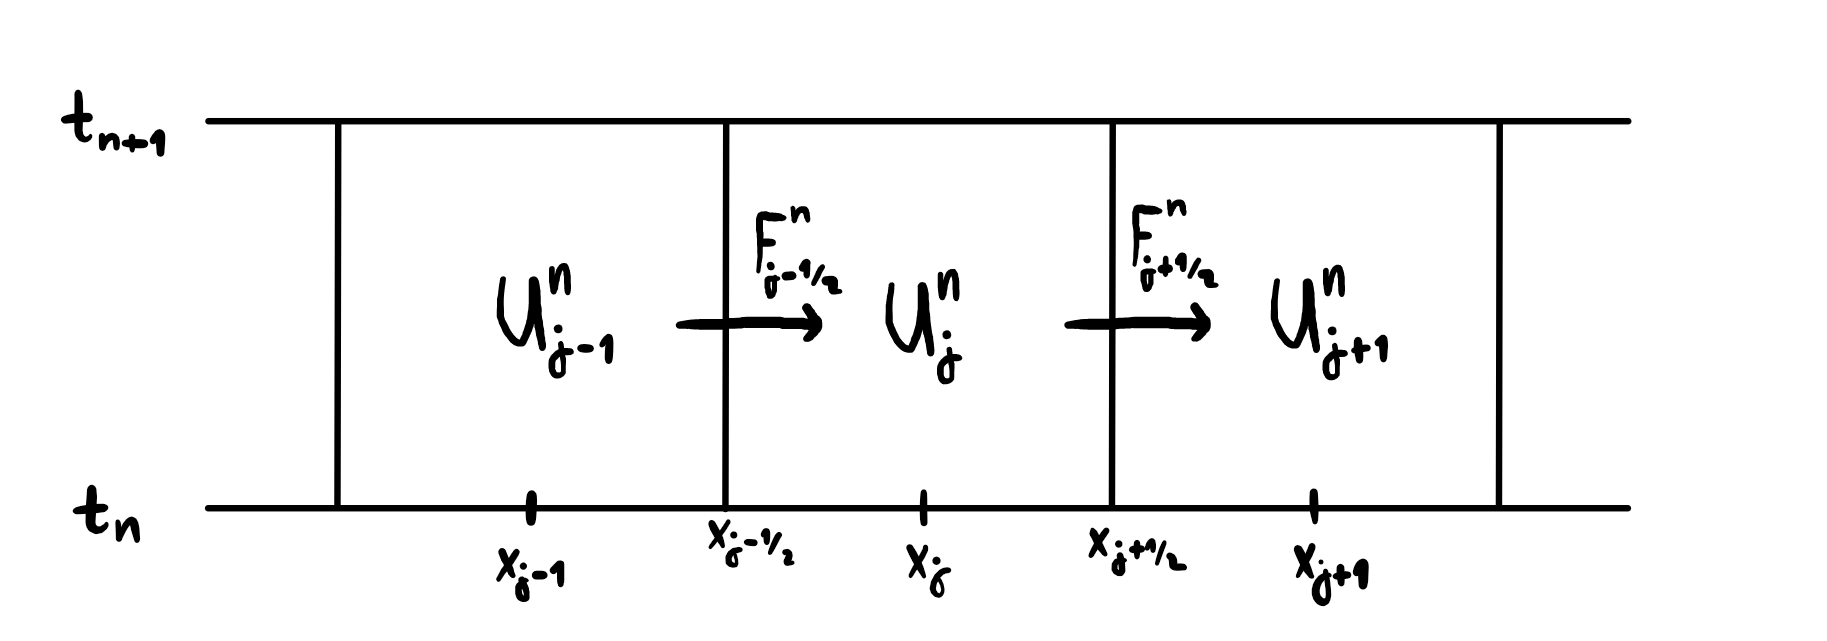
\includegraphics[width=0.90\textwidth]{control_volumes.png}
        \caption{Illustration of the cell averages. Inspired from Fig 4.1, p.65 of \cite{leveque2002}.}
    \end{subfigure}

    \vspace{\floatsep}

    \begin{subfigure}{0.8\textwidth}
        \centering
        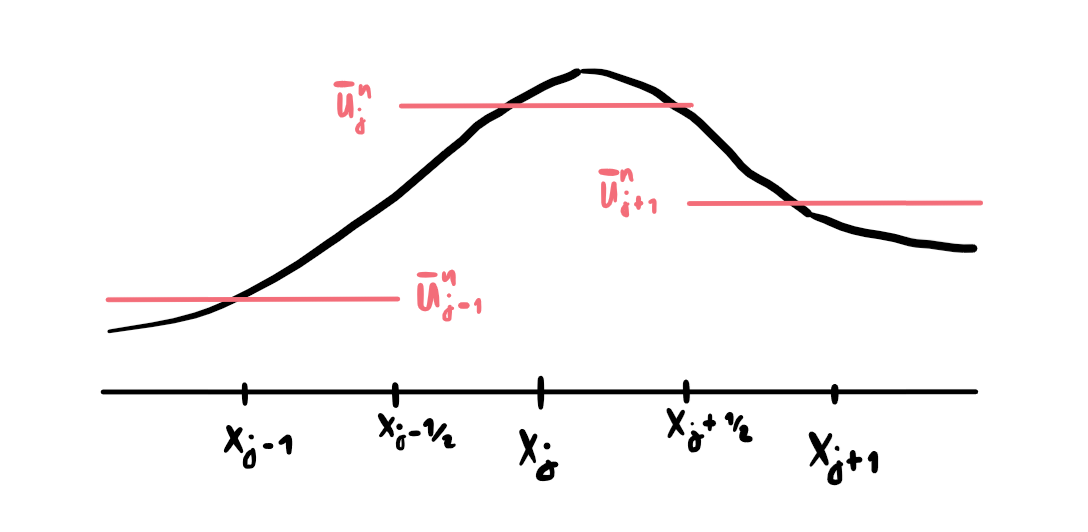
\includegraphics[width=0.90\textwidth]{step-wise_approx.png}
        \caption{Illustration of the step-wise nature the cell-average approximation to $u(x_j,t_n)$ has. Inspired from Fig 17.9, p.418 of \cite{iserles2009}.}
    \end{subfigure}
    \caption{}
\end{figure}

The goal of a successful numerical scheme then is to accurately model the flux through the boundaries of each cell. Explicitly, we want to find some numerical flux function $\mathcal{F}$ so that 
\[
    \mathcal{F}(U_j^n, U_{j+1}^n) \approx \frac{1}{\Delta t} \int_{t_n}^{t_{n+1}} f(u(x_{j+1/2}, t)) dt \qquad \mathcal{F}(U_{j-1}^n, U_{j}^n) \approx \frac{1}{\Delta t} \int_{t_n}^{t_{n+1}} f(u(x_{j-1/2}, t)) dt.
\]

To this end, we say that a numerical method is in \emph{conservation form} if 
\[
    U_j^{n+1} = U_j^n - \frac{\Delta t}{\Delta x} \left[ \mathcal{F}(U_{j}^{n}, U_{j+1}^{n}) - \mathcal{F}(U_{j-1}^{n}, U_{j}^{n}) \right].
\]
Note that while this derivation comes about through the introduction of control volumes, and hence falls under the umbrella of \emph{finite volume methods}, we can also understand it through the lens of finite differences. Specifically, from (2) we get the relation
\[
    \frac{U_j^{n+1} - U_j^n}{\Delta t} + \frac{F_{j+1/2}^n - F_{j-1/2}^n}{\Delta x} = 0
\]
where $F_{j\pm1/2}^n \sim \mathcal{F}$ as before. Hence these methods can be understood to be first-order accurate in time and `somewhat' second-order accurate in space. We say `somewhat' because the reality is complicated.

% bibliography
\nocite{choksi2022}
\nocite{iserles2009}
% \nocite{kutz2013}
% \nocite{trefethen2001}
% \nocite{learncfd}
% \nocite{evans2010}
\nocite{leveque1992}
\nocite{leveque2002}
\printbibliography

\end{document}